\documentclass[11pt,a4paper]{article}
\usepackage[utf8]{inputenc}
\usepackage[T1]{fontenc}
\usepackage{amsfonts}
\usepackage[french]{babel}
\frenchbsetup{StandardLists=true} % à inclure si on utilise \usepackage[francais]{babel}
\usepackage{enumitem}
\usepackage{amssymb}
\usepackage{amsmath}
\usepackage{parskip}
\usepackage[left=2cm,right=2cm,top=2cm,bottom=2cm]{geometry}
\usepackage{multirow}
\usepackage[dvipsnames]{xcolor}

\usepackage[T1]{fontenc}
\usepackage{fouriernc}
\usepackage{graphicx}

\usepackage{setspace}
\singlespacing

\usepackage{pstricks}
\usepackage{xkeyval}
\usepackage{pst-labo}


\usepackage{multicol}
\usepackage{caption}
\usepackage{fancyhdr}
\pagestyle{fancy}
\renewcommand\headrulewidth{1pt}
\fancyhead[L]{Lycée Denis Diderot }
\fancyhead[R]{Classe de Terminale}
\setcounter{page}{7}\fancyfoot[C]{page \thepage}
\fancyfoot[R]{Année 2025 2026}
\fancyfoot[L]{Alexis RUIZ}
\usepackage{multirow,tabularx,booktabs}
\newcommand{\cadreblanc}[1]{%
\medskip\framebox[\linewidth][c]{%
\rule{0mm}{#1mm}}\par
\medskip}

\usepackage{awesomebox}
\setlength{\aweboxvskip}{0mm}
\usepackage{pifont}
\usepackage{chemmacros}
\usepackage{chemist}
\chemsetup{modules=all}

\renewcommand{\arraystretch}{2}
\newcommand*\acocher{\quitvmode{\fboxsep0pt \fboxrule0.8pt \fbox{\vrule height1.8ex depth.1ex width0pt \vrule height0pt depth0pt width1.9ex }}}
\usepackage{colortbl}

\newcommand{\defproblem}{\awesomebox[black]{2pt}{\rotatebox{90}{\large{\textbf{Problématique}}}}{black}}
\newcommand{\defconclusion}{\awesomebox[black]{2pt}{\rotatebox{90}{\Large{\textbf{Conclusion}}}}{black}}
\newcommand{\defbox}{\awesomebox[black]{2pt}{
\includegraphics[scale=0.5]{images/appel exam.png}}{black}}


\frenchbsetup{StandardLists=true}
\begin{document}



\begin{center}
\LARGE{Révision- Prévoir une réaction d'oxydo-réduction}\\[5mm]
\end{center}
\normalsize

\hrule
\vspace {8 mm}

\textbf{Exercices :} Dans un bêcher on plonge un métal dans une solution ionique métallique. 
 Pour chacune des expérience, indiquer s'il y a une réaction, dans ce cas écrire les demi-équations d'oxydo-réduction, puis l'équation de réaction.Si la réaction n'a pas lieu, pas besoin d'écrire les équations.   \\[5mm]

\textbf{Exp~~\ding{202} :} On introduit de la grenaille d'argent (\ch{Ag}) dans une solution contenant des ions Fer (\ch{Fe\pch[]})

\begin{figure}[h]
\begin{minipage}{0.2\textwidth}
\begin{center}
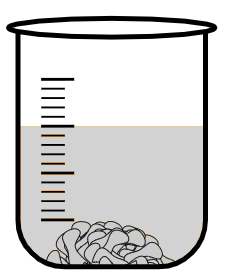
\includegraphics[scale=0.25]{images/sol etain metal al.png} 
\end{center}
\end{minipage}%
\begin{minipage}{0.8\textwidth}
La réaction a-t-elle lieu ? $\Box$ oui $\Box$ non \\[2mm]
Écrire les deux demi équations correspondantes à cette réaction. \\[2mm]
\LARGE{\fbox{$~~~~~~~~ ~~~~~~\longrightarrow~~~~~~~~~~ ~~~~~~~~$} ~~~~~~~~ \fbox{$~~~~~~~~ ~~~~~~~~ \longrightarrow ~~~~~~~~~~~~ $}}\\[2mm]
\normalsize
Écrire l'équation de la réaction. \\[2mm]
\fbox{\LARGE {$~~~~~~~~~~+ ~~~~~~~~~~ \longrightarrow~~~~~~~~~~+ ~~~~~~~~ $}}\\

\end{minipage}
\end{figure}

\vspace {5mm}

\textbf{Exp~~\ding{203} :} On introduit de la grenaille de Zinc (\ch{Zn)} dans une solution contenant des ions nickel (\ch{Ni\pch[2]})
\begin{figure}[h]
\begin{minipage}{0.7\textwidth}
La réaction a-t-elle lieu ? $\Box$ oui $\Box$ non \\[2mm]
Écrire les deux demi équations correspondantes à cette réaction. \\[2mm]
\LARGE{\fbox{$~~~~~~~~ ~~~~~~\longrightarrow~~~~~~~~~~ ~~~~~~~~$} ~~~~~~~~ \fbox{$~~~~~~~~ ~~~~~~~~ \longrightarrow ~~~~~~~~~~~~ $}}\\[2mm]
\normalsize
Écrire l'équation de la réaction. \\[2mm]
\fbox{\LARGE {$~~~~~~~~~~+ ~~~~~~~~~~ \longrightarrow~~~~~~~~~~+ ~~~~~~~~ $}}\\

\end{minipage}
\begin{minipage}{0.3\textwidth}
\begin{center}
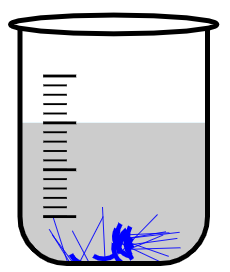
\includegraphics[scale=0.25]{images/sol Al metal Fe.png} 
\end{center}
\end{minipage}%
\end{figure}

\vspace {5mm}

\textbf{Exp~~\ding{204} :} On introduit une bague en or (\ch{Au}) dans une solution contenant des ions étain (\ch{Sn\pch[2]})
\begin{figure}[h]
\begin{minipage}{0.3\textwidth}
\begin{center}
\includegraphics[scale=0.25]{images/sol etain metal Al.png} 
\end{center}
\end{minipage}%
\begin{minipage}{0.8\textwidth}
La réaction a-t-elle lieu ? $\Box$ oui $\Box$ non \\[2mm]
Écrire les deux demi équations correspondantes à cette réaction. \\[2mm]
\LARGE{\fbox{$~~~~~~~~ ~~~~~~\longrightarrow~~~~~~~~~~ ~~~~~~~~$} ~~~~~~~~ \fbox{$~~~~~~~~ ~~~~~~~~ \longrightarrow ~~~~~~~~~~~~ $}}\\[2mm]
\normalsize
Écrire l'équation de la réaction. \\[2mm]
\fbox{\LARGE {$~~~~~~~~~~+ ~~~~~~~~~~ \longrightarrow~~~~~~~~~~+ ~~~~~~~~ $}}\\

\end{minipage}
\end{figure}


\textbf{Exp~~\ding{205} :} On introduit de la grenaille d étain(\ch{Sn})  dans une solution contenant des ions fer (\ch{Fe\pch[2]})
\begin{figure}[h!]
\begin{minipage}{0.7\textwidth}
La réaction a-t-elle lieu ? $\Box$ oui $\Box$ non \\[2mm]
Écrire les deux demi équations correspondantes à cette réaction. \\[2mm]
\LARGE{\fbox{$~~~~~~~~ ~~~~~~\longrightarrow~~~~~~~~~~ ~~~~~~~~$} ~~~~~~~~ \fbox{$~~~~~~~~ ~~~~~~~~ \longrightarrow ~~~~~~~~~~~~ $}}\\[2mm]
\normalsize
Écrire l'équation de la réaction. \\[2mm]
\fbox{\LARGE {$~~~~~~~~~~+ ~~~~~~~~~~ \longrightarrow~~~~~~~~~~+ ~~~~~~~~ $}}\\

\end{minipage}
\begin{minipage}{0.3\textwidth}
\begin{center}
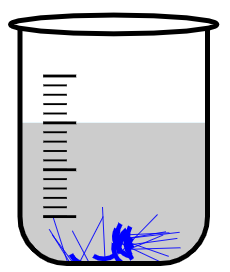
\includegraphics[scale=0.25]{images/sol Al metal Fe.png} 
\end{center}
\end{minipage}%
\end{figure}


\newpage

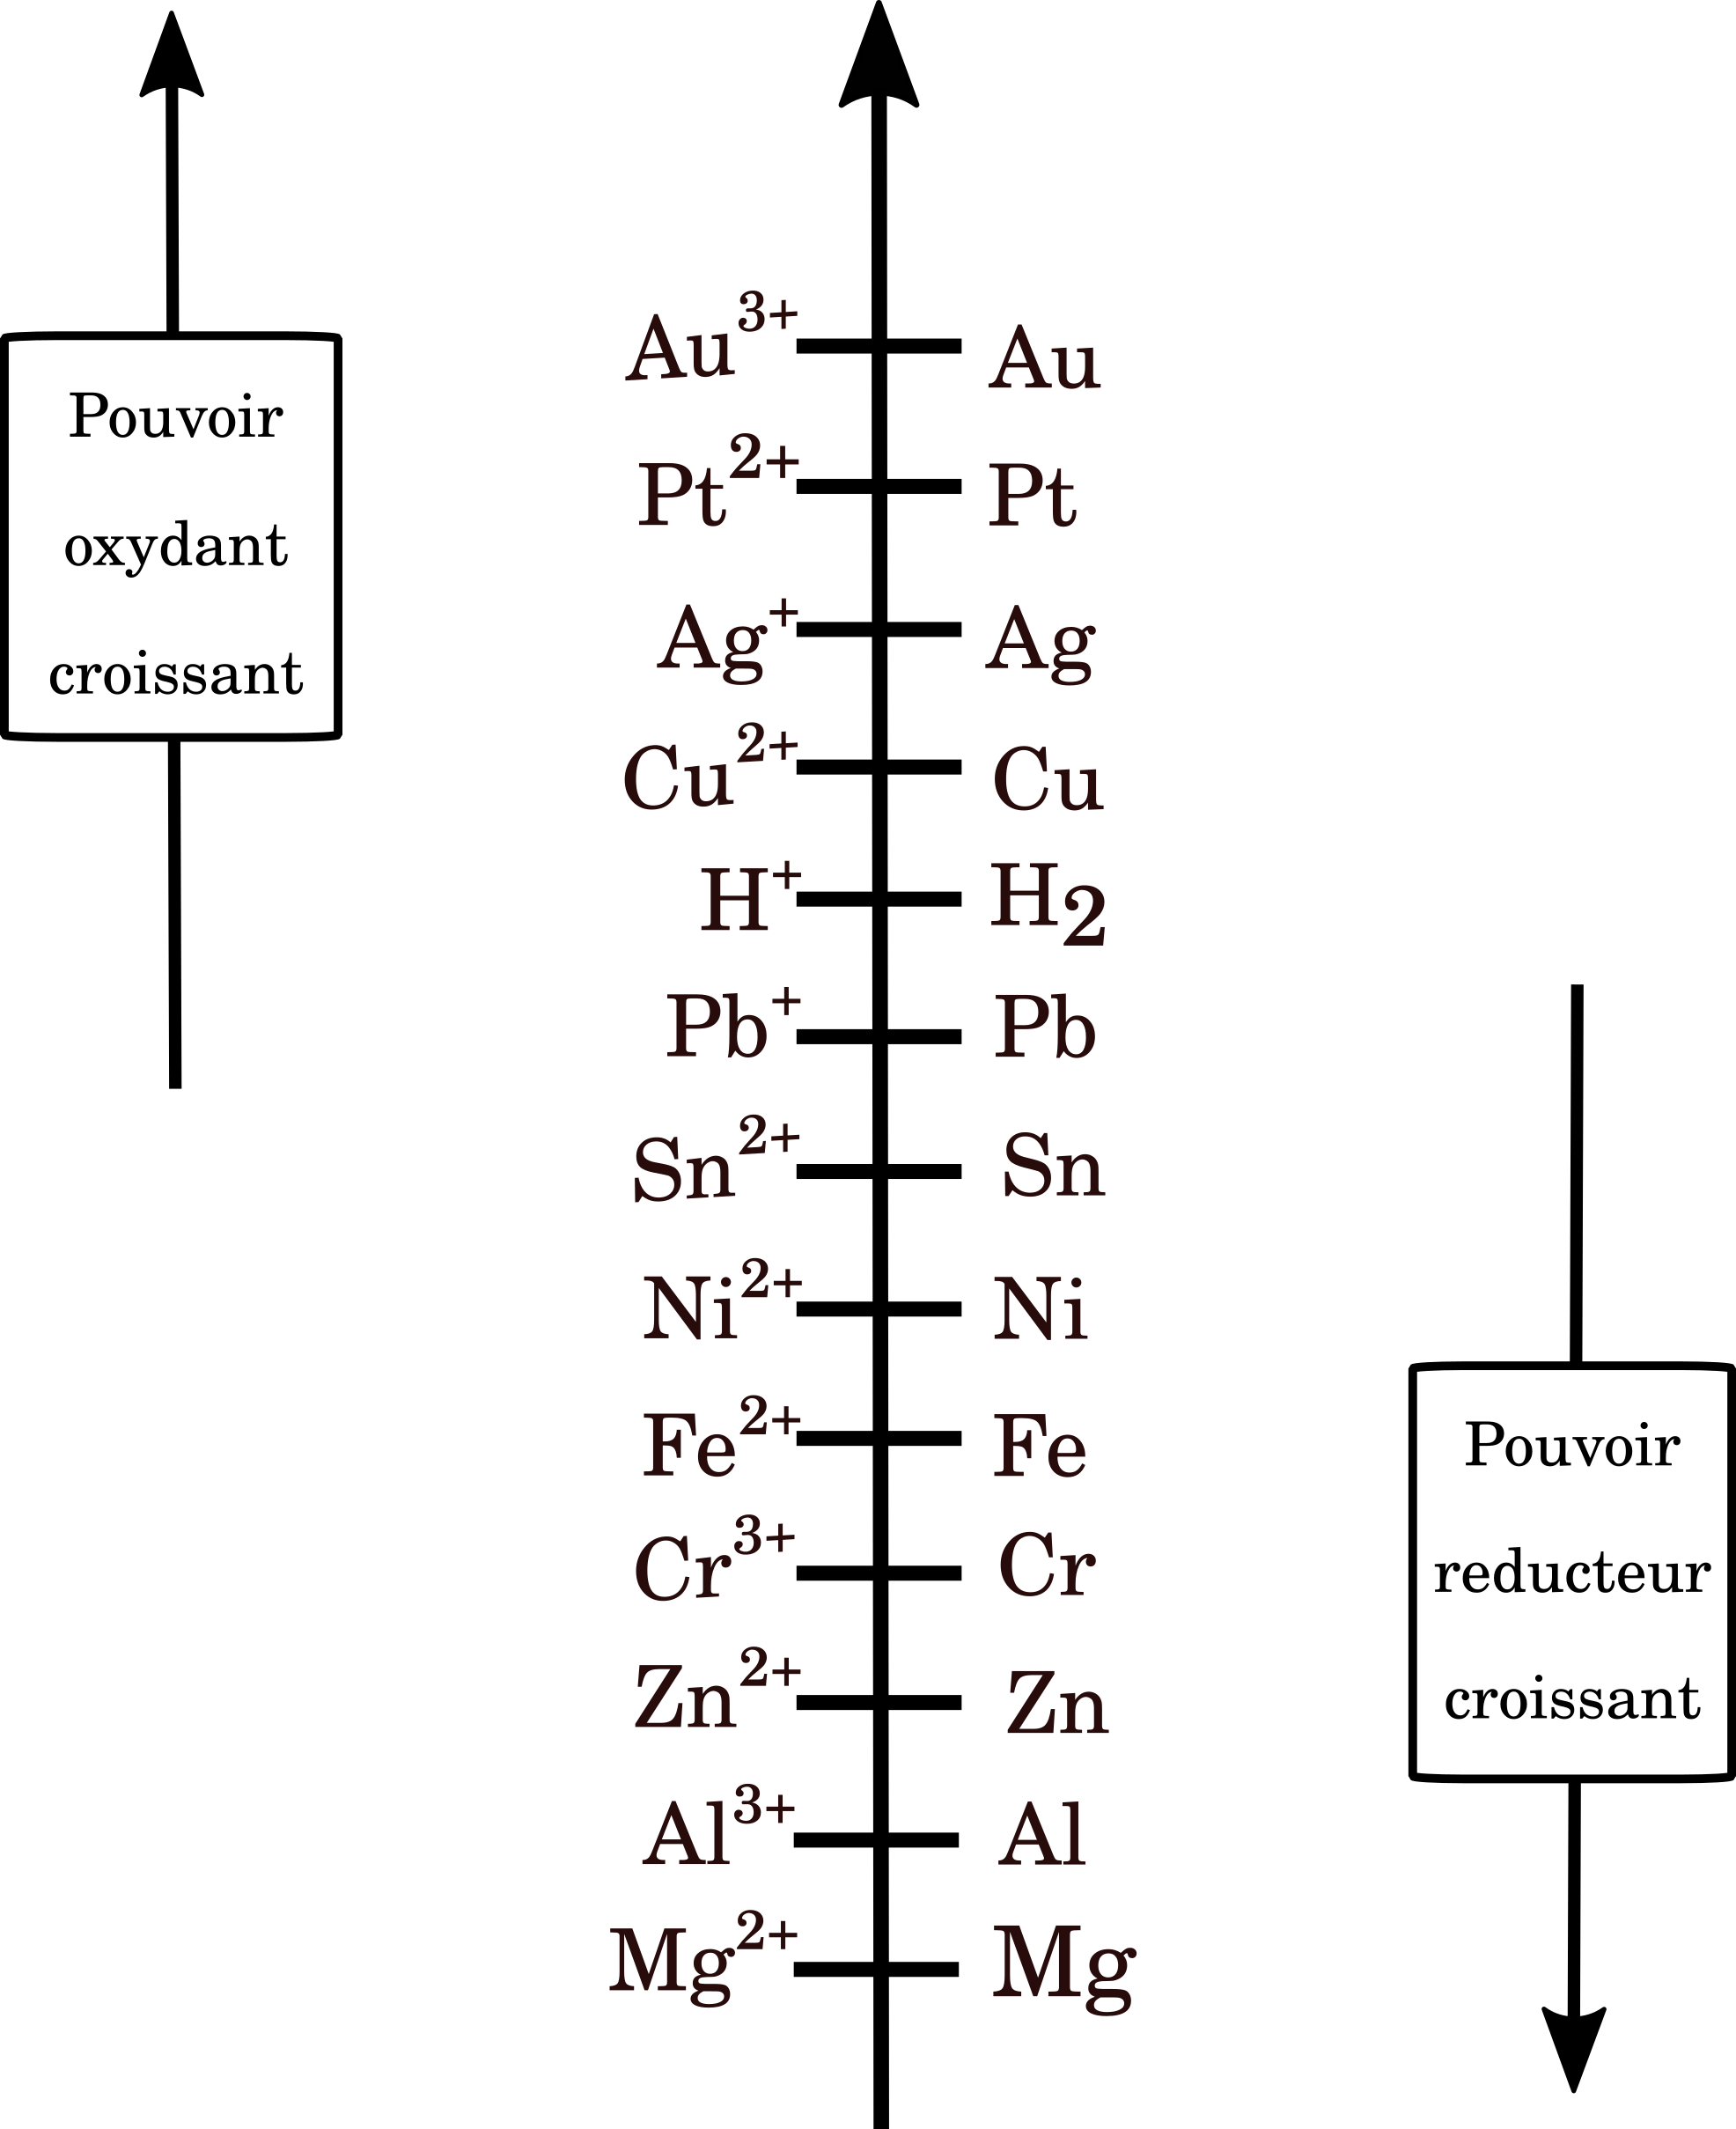
\includegraphics[]{images/classification.png}






\end{document}